% Editable vector artwork for the JSS manuscript: the 2x2 contextual-input x sharing design.
% Rebuild from manuscript/jss/figures/ with:
%   tectonic -X compile framework_2x2.tex
% The resulting PDF is included at text width; no raster assets are used.
\documentclass[tikz,border=2pt]{standalone}
\usepackage[T1]{fontenc}
\usepackage{amsmath}
\usetikzlibrary{arrows.meta}
\renewcommand{\familydefault}{\sfdefault}

\begin{document}
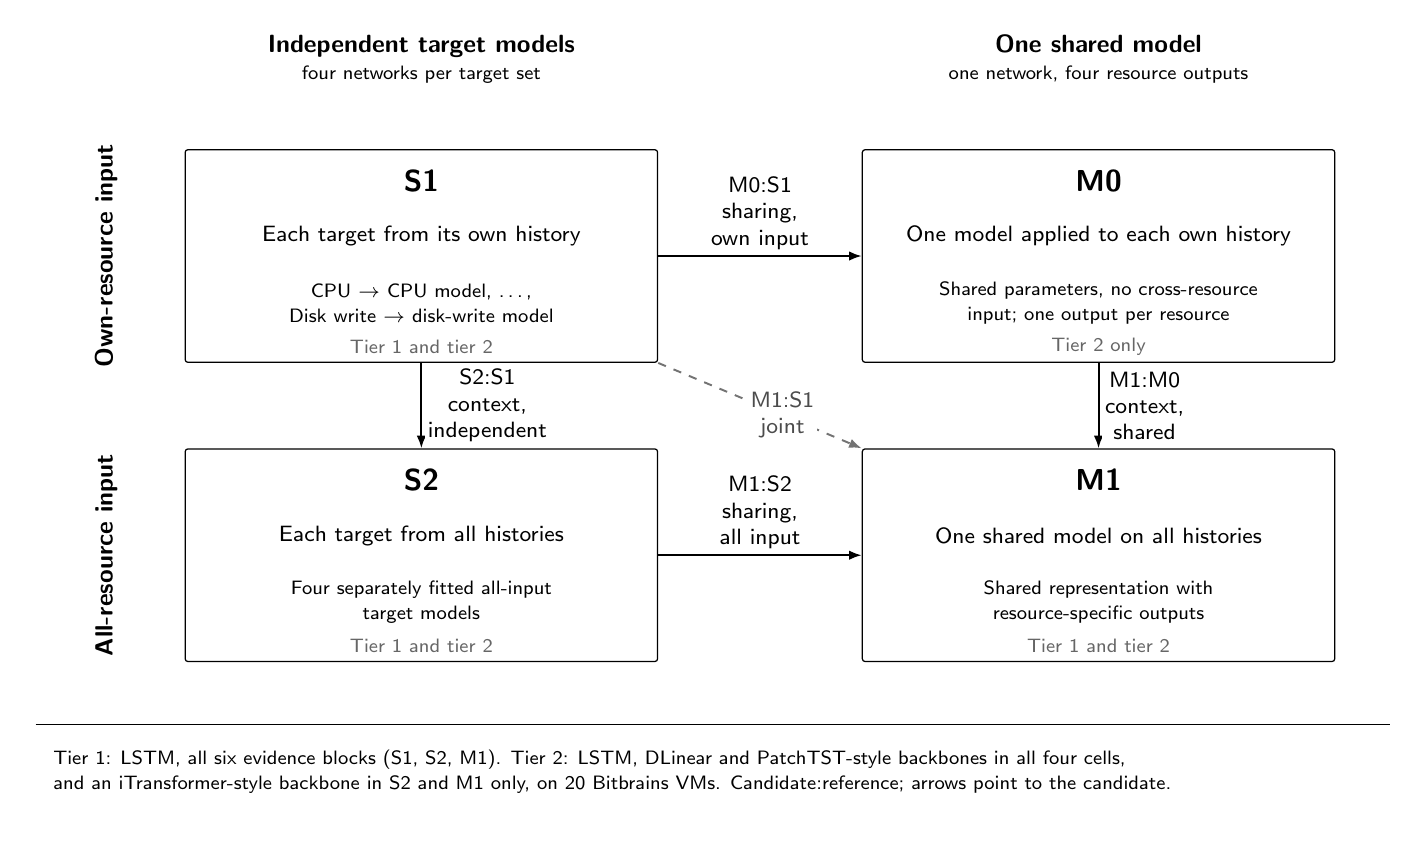
\begin{tikzpicture}[
  x=1mm,y=1mm,
  font=\fontsize{8.5}{10}\selectfont,
  line width=0.45pt,
  flow/.style={-{Latex[length=1.6mm,width=1.2mm]},line width=0.7pt},
  cell/.style={draw,rectangle,rounded corners=1pt,align=center,minimum width=60mm,minimum height=27mm,
               inner sep=2pt},
  heading/.style={font=\fontsize{11}{12}\selectfont\bfseries},
  axis/.style={font=\fontsize{9}{10.5}\selectfont\bfseries,align=center},
  note/.style={font=\fontsize{7.5}{9}\selectfont,align=center},
  contrast/.style={font=\fontsize{8}{9.5}\selectfont,align=center,fill=white,inner sep=1pt}
]
  \path[use as bounding box] (0,-14) rectangle (174,86);

  % Axis headings.
  \node[axis] at (50,82) {Independent target models\\[-1pt]{\normalfont\fontsize{7.5}{9}\selectfont four networks per target set}};
  \node[axis] at (136,82) {One shared model\\[-1pt]{\normalfont\fontsize{7.5}{9}\selectfont one network, four resource outputs}};
  \node[axis,rotate=90] at (10,57) {Own-resource input};
  \node[axis,rotate=90] at (10,19) {All-resource input};

  % Cells.
  \node[cell] (s1) at (50,57) {};
  \node[cell] (m0) at (136,57) {};
  \node[cell] (s2) at (50,19) {};
  \node[cell] (m1) at (136,19) {};

  \node[heading] at (50,66.5) {S1};
  \node at (50,59.5) {Each target from its own history};
  \node[note] at (50,51) {CPU $\rightarrow$ CPU model, \ldots,\\Disk write $\rightarrow$ disk-write model};
  \node[note,text=black!60] at (50,45.5) {Tier 1 and tier 2};

  \node[heading] at (136,66.5) {M0};
  \node at (136,59.5) {One model applied to each own history};
  \node[note] at (136,51) {Shared parameters, no cross-resource\\input; one output per resource};
  \node[note,text=black!60] at (136,45.5) {Tier 2 only};

  \node[heading] at (50,28.5) {S2};
  \node at (50,21.5) {Each target from all histories};
  \node[note] at (50,13) {Four separately fitted all-input\\target models};
  \node[note,text=black!60] at (50,7.5) {Tier 1 and tier 2};

  \node[heading] at (136,28.5) {M1};
  \node at (136,21.5) {One shared model on all histories};
  \node[note] at (136,13) {Shared representation with\\resource-specific outputs};
  \node[note,text=black!60] at (136,7.5) {Tier 1 and tier 2};

  % Sharing contrasts (horizontal) and context contrasts (vertical).
  \draw[flow] (s1.east) -- node[contrast,above=1pt] {M0:S1\\sharing,\\own input} (m0.west);
  \draw[flow] (s2.east) -- node[contrast,above=1pt] {M1:S2\\sharing,\\all input} (m1.west);
  \draw[flow] (s1.south) -- node[contrast,right=1pt] {S2:S1\\context,\\independent} (s2.north);
  \draw[flow] (m0.south) -- node[contrast,right=1pt] {M1:M0\\context,\\shared} (m1.north);
  \draw[flow,dashed,black!55] (s1.south east) to[bend left=0] node[contrast,pos=0.62,text=black!70] {M1:S1\\joint} (m1.north west);

  % Footer: backbones and design-defined cells.
  \draw (1,-2.5) -- (173,-2.5);
  \node[note,anchor=west,align=left] at (2,-8.5)
    {Tier 1: LSTM, all six evidence blocks (S1, S2, M1). Tier 2: LSTM, DLinear and PatchTST-style backbones in all four cells,\\
     and an iTransformer-style backbone in S2 and M1 only, on 20 Bitbrains VMs. Candidate:reference; arrows point to the candidate.};
\end{tikzpicture}
\end{document}
